Se realizo un diagrama de Gantt acorde a la Tabla (\ref{tab:tareas}). En este se marcó el camino crítico en rojo.
\begin{figure}[H]
	\centering
	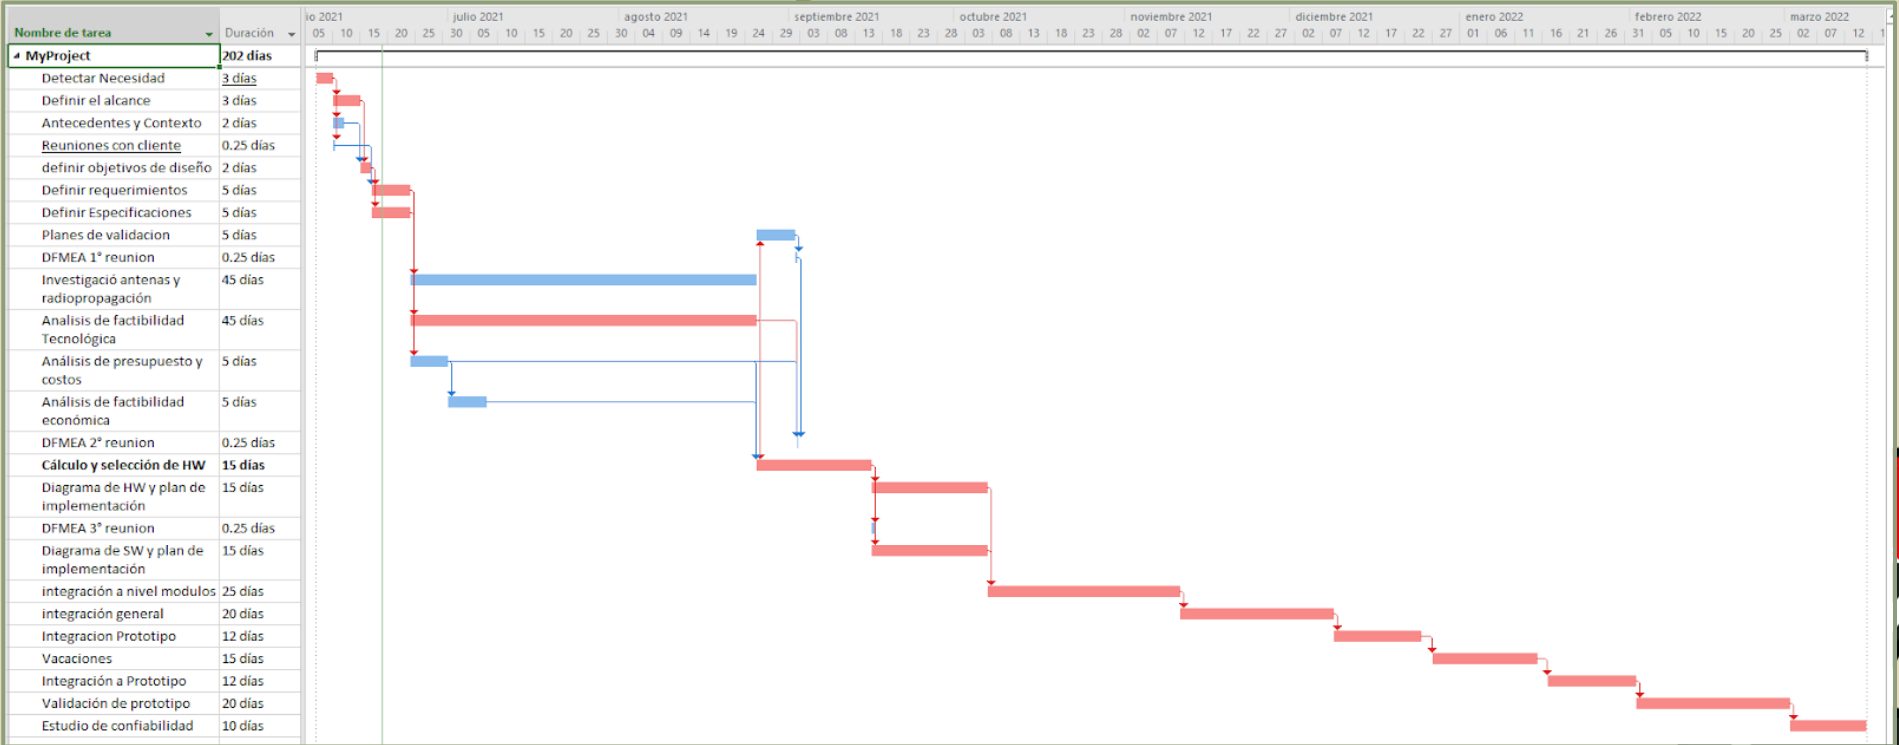
\includegraphics[width=1\linewidth]{ImagenesFactibilidad/project}
	\caption{Diagrama de Gantt del proyecto.}
	\label{fig:gantt}
\end{figure}

Luego se realizó una simulación de Montecarlo utilizando la distribución $\beta$ para las variables aleatorias, obteniendo como resultado el análisis plasmado en la Figura (\ref{fig:montecarlo_tiempos}). Se tiene en cuenta que por teorema central del límite la suma de las variables aleatorias $\beta$ convergen a una normal.

En este gráfico se ve la probabilidad de terminar el proyecto en un intervalo de entre 1533 a 1957 horas, con una probabilidad del 95\%. Esta distribución es el lapso entre que se comienza el proyecto y se termina, a través del camino crítico.

\begin{figure}[H]
	\centering
	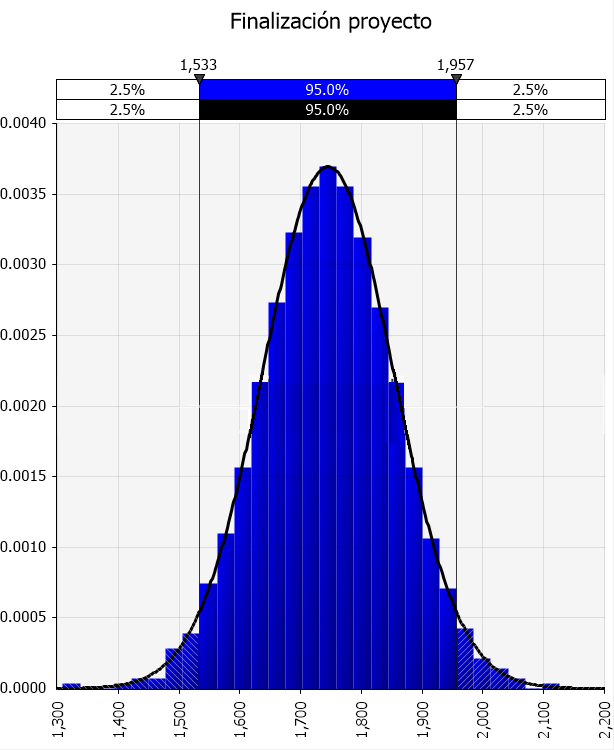
\includegraphics[width=0.5\linewidth]{ImagenesFactibilidad/montecarlo}
	\caption{Simulación de Montecarlo.}	
	\label{fig:montecarlo_tiempos}
\end{figure}


A continuación, se muestran la cantidad de horas de ingeniería total. Para obtener los resultados de la Figura (\ref{fig:montecarlo_tiempos_ing}), se tuvieron cuenta la paralelización de actividades y la disponibilidad de 4 trabajadores.
\begin{figure}[H]
	\centering
	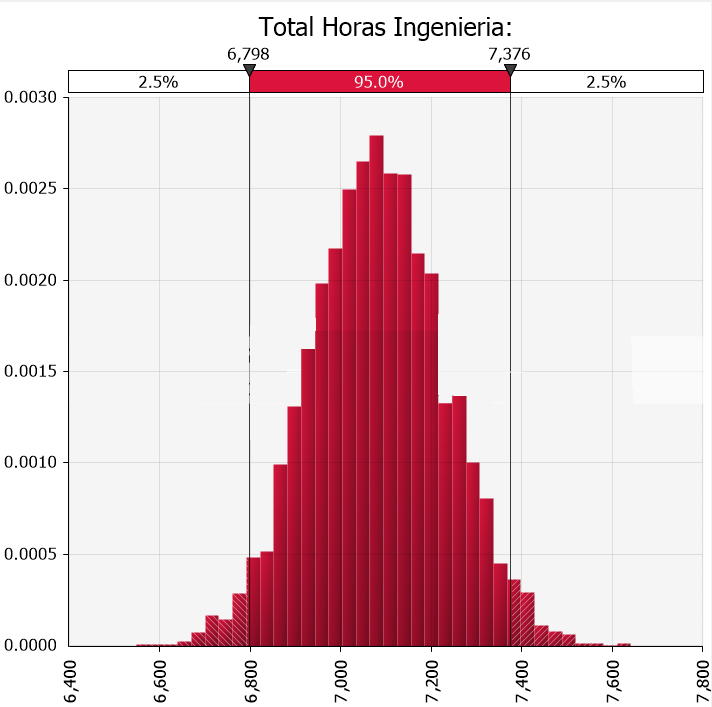
\includegraphics[width=0.5\linewidth]{ImagenesFactibilidad/montecarlo_tiempo_largo}	
	\caption{Simulación de Montecarlo para tiempo de ingeniería.}
	\label{fig:montecarlo_tiempos_ing}
\end{figure}

Se puede observar que el tiempo total de horas de ingeniería corresponde a un rango entre aproximadamente 6800 a 7400 horas, con una media de aproximadamente 7100 horas.